% !TeX root = ../../main.tex

\begin{figure}[h!]
	\centering
	\begin{subfigure}[b]{0.3\textwidth}
		\centering
		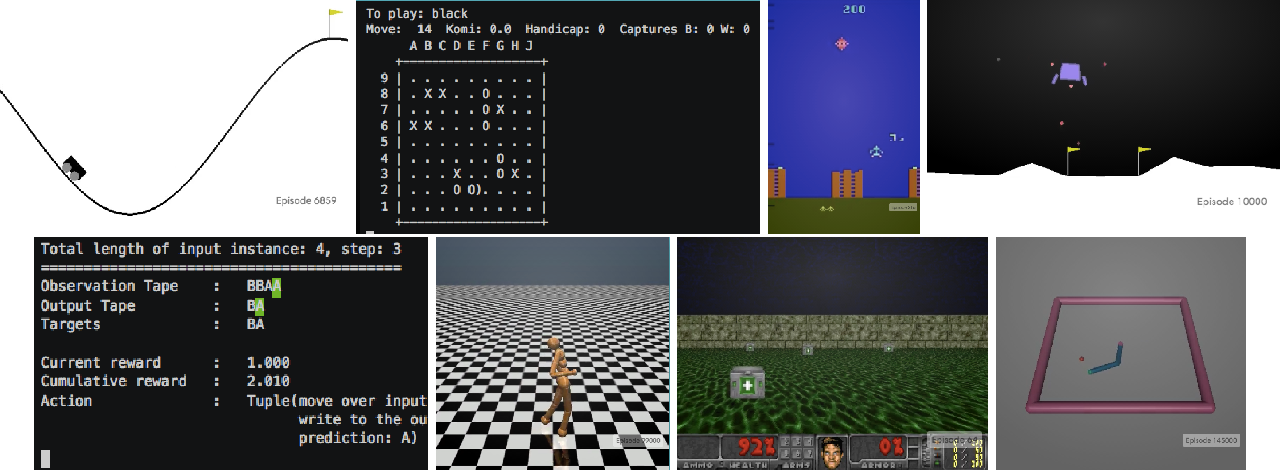
\includegraphics[width=0.7\textwidth]{figures/existing_envs/openai_gym}
		\caption{OpenAI Gym}
		\label{fig:openai_gym}
	\end{subfigure}
	\hfill
	\begin{subfigure}[b]{0.3\textwidth}
		\centering
		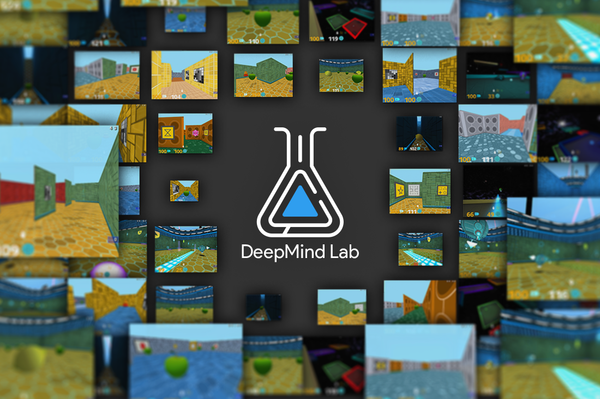
\includegraphics[width=0.7\textwidth]{figures/existing_envs/deepmind_lab.png}
		\caption{DeepMind Lab}
		\label{fig:deepmind_lab}
	\end{subfigure}
	\hfill
	\begin{subfigure}[b]{0.3\textwidth}
		\centering
		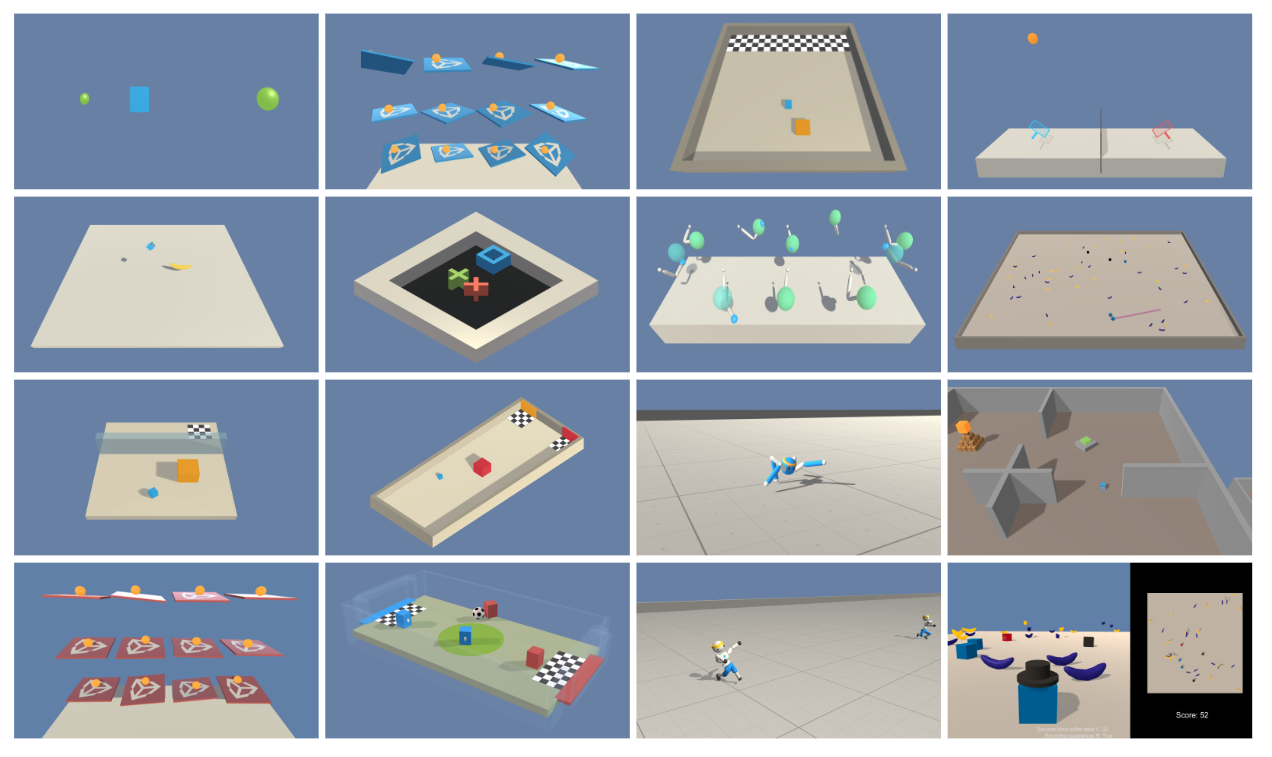
\includegraphics[width=0.7\textwidth]{figures/existing_envs/unity_mlagents.png}
		\caption{Unity MLAgents}
		\label{fig:unity_mlagents}
	\end{subfigure}
	\hfill
	
	\begin{subfigure}[b]{0.3\textwidth}
		\centering
		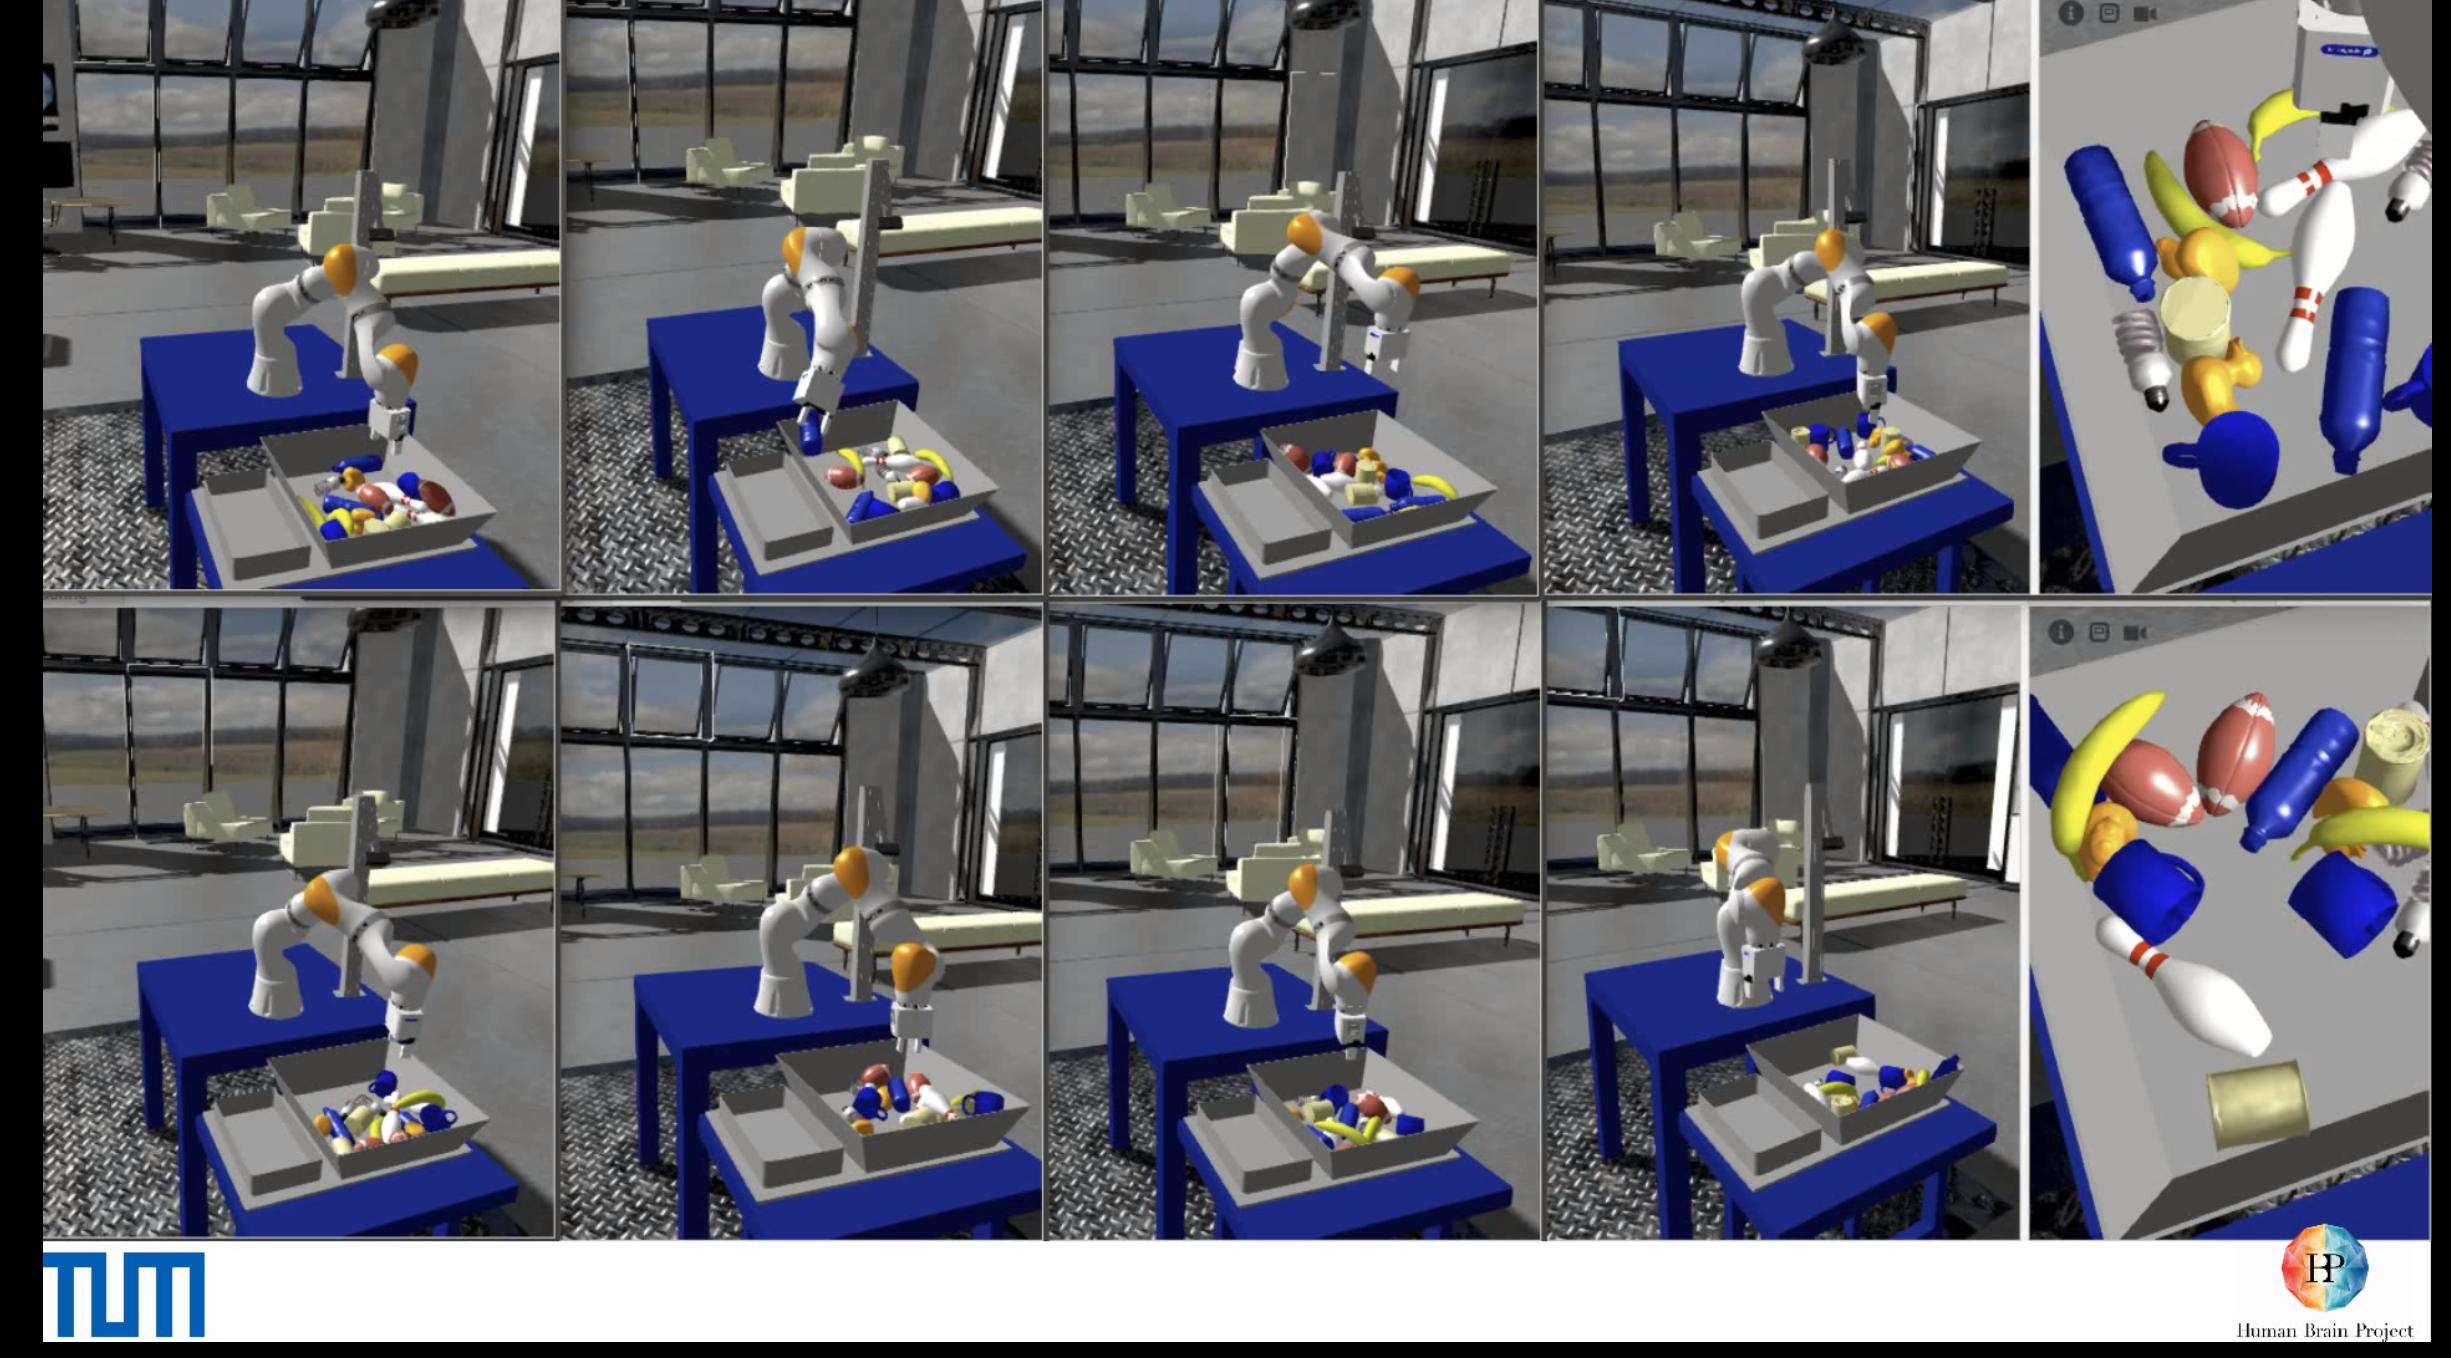
\includegraphics[width=0.7\textwidth]{figures/existing_envs/nrp.png}
		\caption{Neurorobotics Platform}
		\label{fig:atari_2600}
	\end{subfigure}
	\hfill
	\begin{subfigure}[b]{0.3\textwidth}
		\centering
		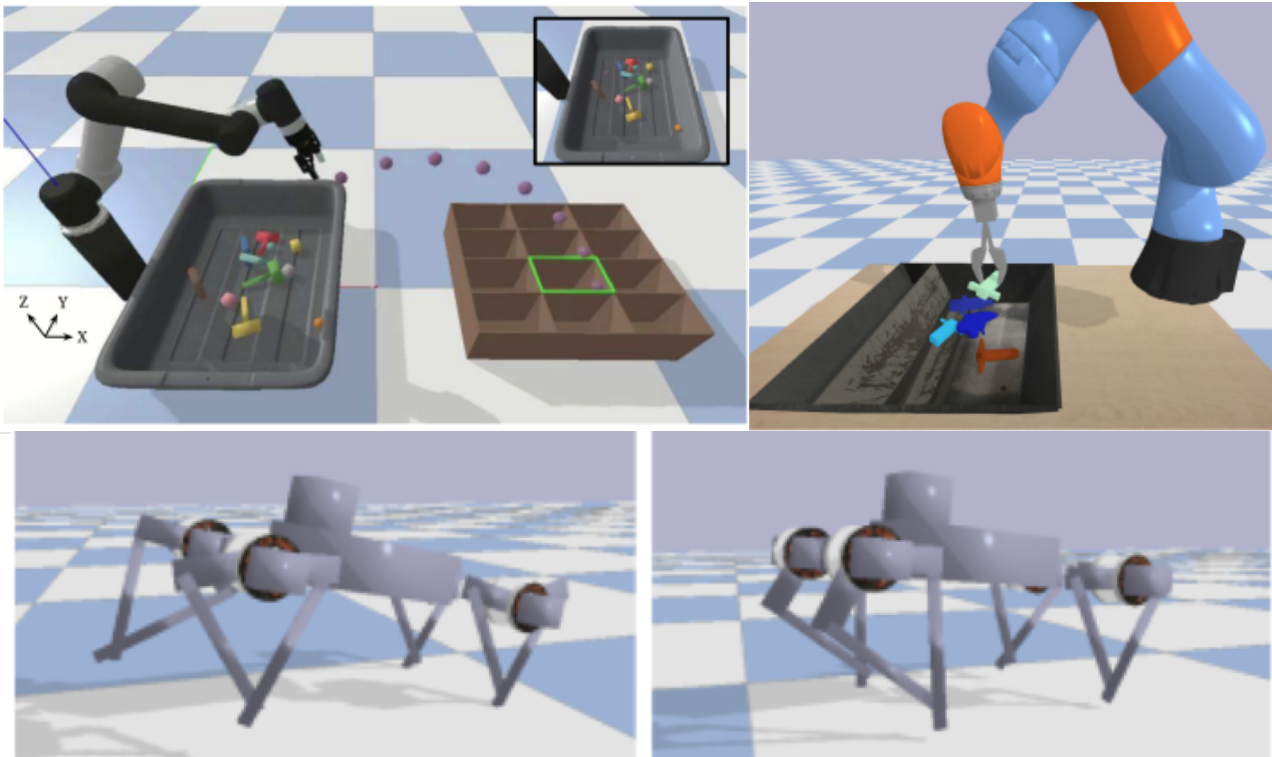
\includegraphics[width=0.7\textwidth]{figures/existing_envs/pybullet.png}
		\caption{PyBullet}
		\label{fig:pybullet}
	\end{subfigure}
	\hfill
	\begin{subfigure}[b]{0.3\textwidth}
		\centering
		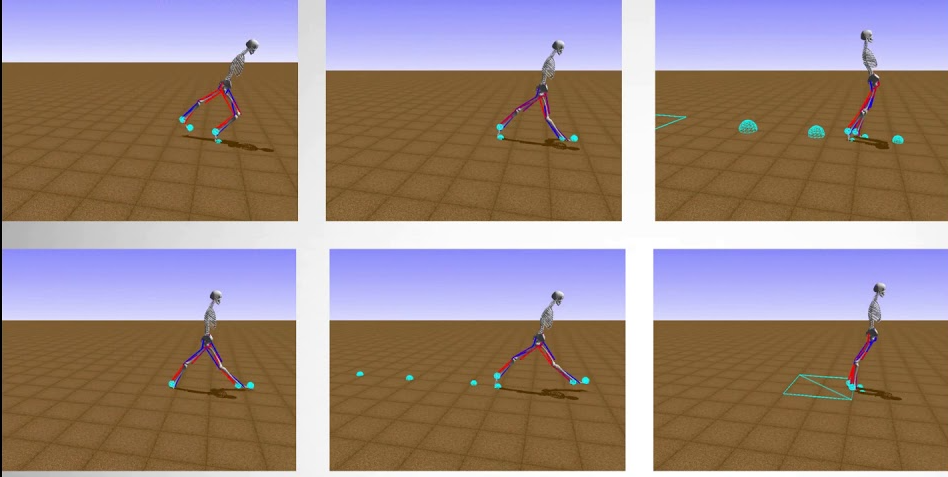
\includegraphics[width=0.7\textwidth]{figures/existing_envs/osim_rl.png}
		\caption{Osim RL: musculoskeletal models in OpenSim}
		\label{fig:osim_rl}
	\end{subfigure}
	
	\begin{subfigure}[b]{0.3\textwidth}
		\centering
		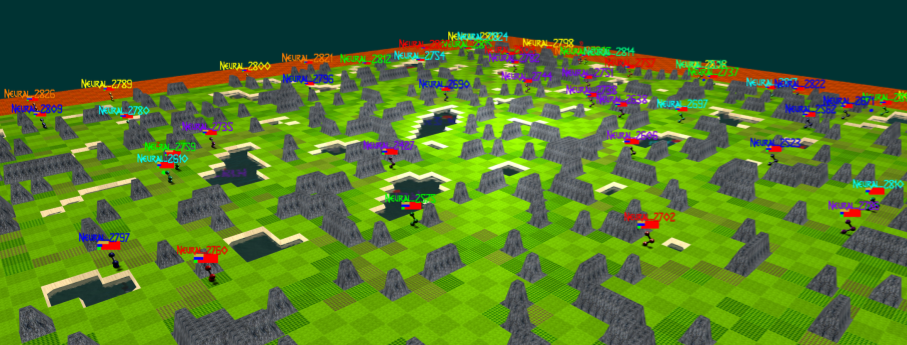
\includegraphics[width=0.7\textwidth]{figures/existing_envs/openai_mmo.png}
		\caption{OpenAI MML}
		\label{fig:openai_mmo}
	\end{subfigure}
	\hfill
	\begin{subfigure}[b]{0.3\textwidth}
		\centering
		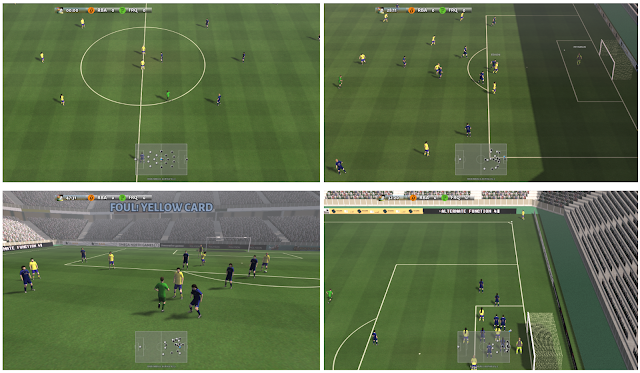
\includegraphics[width=0.7\textwidth]{figures/existing_envs/google_football.png}
		\caption{Google Research Football}
		\label{fig:google_football}
	\end{subfigure}
	\hfill
	\begin{subfigure}[b]{0.3\textwidth}
		\centering
		\includegraphics[width=0.7\textwidth]{figures/existing_envs/deepmind_alphstar.png}
		\caption{StarCraft II Learning Environment}
		\label{fig:deepmind_alphstar}
	\end{subfigure}
	\hfill
	\caption{Examples of existing Deep RL Environments}
	\label{fig:envs_examples}
\end{figure}